\documentclass[journal,12pt,onecolumn]{IEEEtran}
\usepackage{cite}
\usepackage{caption}
\usepackage{graphicx}
\usepackage{amsmath,amssymb,amsfonts,amsthm}
\usepackage{algorithmic}
\usepackage{graphicx}
\usepackage{textcomp}
\usepackage{xcolor}
\usepackage{tfrupee}
\usepackage{txfonts}
\usepackage{listings}
\usepackage{enumitem}
\usepackage{mathtools}
\usepackage{gensymb}
\usepackage{comment}
\usepackage[breaklinks=true]{hyperref}
\usepackage{tkz-euclide} 
\usepackage{listings}
\usepackage{gvv}
%\def\inputGnumericTable{}
\usepackage[latin1]{inputenc} 
\usetikzlibrary{arrows.meta, positioning}
\usepackage{xparse}
\usepackage{color}                                            
\usepackage{array}                                            
\usepackage{longtable}                                       
\usepackage{calc}                                             
\usepackage{multirow}
\usepackage{multicol}
\usepackage{hhline}                                           
\usepackage{ifthen}                                           
\usepackage{lscape}
\usepackage{tabularx}
\usepackage{array}
\usepackage{float}
\usepackage{marvosym}
\usepackage{float}
%\newcommand{\define}{\stackrel{\triangle}{=}}
\theoremstyle{remark}
\usepackage{circuitikz}
\captionsetup{justification=centering}
\usepackage{tikz}

\title{Matrices in Geometry 8.4.40}
\author{EE25BTECH11037 - Divyansh}
\begin{document}
\vspace{3cm}
\maketitle
{\let\newpage\relax\maketitle}
\textbf{Question: }
Let $\vec{P}$ be a point on the ellipse $\frac{x^2}{a^2} + \frac{y^2}{b^2}=1 , 0<b<a$. Let the line parallel to the X axis passing through $\vec{P}$ meet the circle $x^2 + y^2= a^2$ at the point $\vec{Q}$ such that $\vec{P}$ and $\vec{Q}$ are on the same side of the X axis. For two positive real numbers $r$ and $s$, find the locus of the point $\vec{R}$ on $\vec{P}\vec{Q}$ such that $PR = r$ as $\vec{P}$ varies over the ellipse.
\vspace{2mm}


\textbf{Solution:}
\\
The given ellipse is 
\begin{align}
    \vec{E} \ : \ \vec{x}^{\top}\vec{V}\vec{x} + 2 \vec{u}^{\top}\vec{x} + f=0 \ : \ \vec{V}=\myvec{b^2 & 0 \\ 0 & a^2}, \vec{u}=\myvec{0\\0}\ , \ f=-a^2b^2 \\
    \implies \vec{E} \ : \vec{x}^{\top}\vec{V}\vec{x} + f=0
\end{align}
The line parallel to the X-axis and passing through a point $\vec{P}$ on the ellipse is 
\begin{align}
    \vec{L}\ :\ \vec{n}^{\top} \vec{x} =c \ : \ \vec{n}=\myvec{0\\1} \ , \ c=y_P
\end{align}
$\vec{P}$ satisfies this line; therefore, $c=y_P$

$\vec{R}$ is a point on line $\vec{L}$ and at a distance $r$ from $\vec{P}$
\begin{align}
    \vec{R} - \vec{P}= r\vec{e_1} \implies \vec{P}=\vec{R} - r\vec{e_1}\  ; \ \vec{e_1}=\myvec{1\\0}
\end{align}
Since, $\vec{P}$ is a point on $\vec{E}$
\begin{align}
    \vec{P}^{\top}\vec{V}\vec{P} + f=0
\end{align}
Substituting $\vec{P} = \vec{Q} -r\vec{e_1}$
\begin{align}
    \brak{\vec{R} -r\vec{e_1}}^{\top}\vec{V}\brak{\vec{R} -r\vec{e_1}} + f=0 \implies \vec{R}^{\top}\vec{V}\vec{R} - 2r\vec{R}^{\top}\vec{V}\vec{e_1} + r^2\vec{e_1}^{\top}\vec{V}\vec{e_1}+f=0\\
    \vec{R}= \myvec{x\\y} \ , \ \vec{V}=\myvec{b^2 & 0 \\ 0 & a^2} \ , \ \vec{e_1}=\myvec{1\\0} \ , \ f=-a^2b^2
\end{align}
Thus the locus of the point $\vec{R}$ is
\begin{align}
    \vec{x}^{\top}\vec{V'}\vec{x} + 2 \vec{u'}^{\top}\vec{x} + f'=0 \ : \ \vec{V'}=\vec{V} \ , \ \vec{u'}=\brak{-r\vec{V}\vec{e_1}} \ , \ f'=f+ r^2\vec{e_1}^{\top}\vec{V}\vec{e_1}
\end{align}
Simplifying this equation, we get
\begin{align}
 	\vec{x}^{\top}\vec{V'}\vec{x} + 2\vec{u'}^{\top}\vec{x} +f'=0 \ , \ \vec{V'}=\myvec{b^2 & 0\\0&a^2} \ , \ \vec{u'}=\myvec{-b^2r\\0} \ , \  f'=b^2r^2 - a^2b^2
\end{align}
This is the equation of locus of the point $\vec{R}$, which is an ellipse.
Let us try to draw the locus for $a=4, b=2 , r=1 $
\begin{figure}[H]
        \centering
        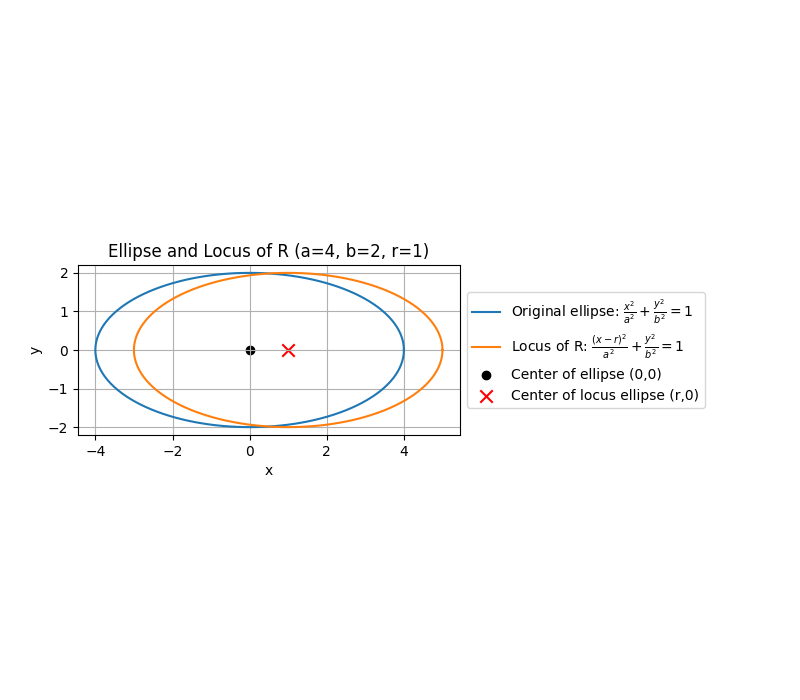
\includegraphics[width=1\columnwidth]{figs/1.png}
        \caption{Figure for 8.4.40 for $a=4, b=2, r=1$}
        \label{fig:placeholder}
    \end{figure}
\end{document}


